%% ------------------------------------------------------------------------- %%
\chapter{Introdução}
\label{cap:introducao}

Test-Driven Development (TDD), ou Desenvolvimento Guiado pelos Testes,
é uma das práticas dentre as sugeridas na Programação
Extrema (XP) \cite{XPExplained}. É baseada em um pequeno ciclo de
desenvolvimento, no qual o desenvolvedor deve sempre escrever um teste antes
mesmo de implementar a funcionalidade esperada, e depois, com o código
passando pelo recém-criado teste, o desenvolvedor deve refatorar para 
remover duplicação de dados e de código \cite{TDDByExample}.
Apesar da constante escrita de testes automatizados, os benefícios da
prática vão além disso. Na opinião de muitos autores conhecidos, TDD promove
uma melhoria significativa no design de classes, auxiliando o programador a
criar classes mais coesas e menos acopladas \cite{TDDByExample} \cite{GOOS} 
\cite{astels-tdd}.

Entender os efeitos de TDD no design de classes é de grande importância para os
desenvolvedores.
Criar classes ou, em um nível maior de abstração, módulos que possuam um baixo
acoplamento e uma alta coesão demandam um esforço muito grande do desenvolvedor. 
É muito comum, após algum tempo de desenvolvimento, o design perder qualidade
e qualquer tipo de manutenção torna-se difícil e, por consequência, custosa.
Muitas práticas objetivam reduzir esses problemas, como programação pareada ou
revisão de código. Os praticantes de TDD acreditam que os testes sejam uma outra
maneira de validar o design criado, e utilizam esse feedback para melhorá-lo.

Em um questionário de 2010 para descobrir que práticas eram feitas por times
ágeis \cite{wambler-survey-agile}, Scott Ambler mostrou que 53\% dos times ágeis
adotaram TDD como uma maneira para validar o trabalho feito, conforme mostra a 
Figura \ref{fig:wambler-agile-2010}. Outro questionário, de 2008, também realizado por Ambler
\cite{wambler-survey-tdd}, focado em TDD, mostra que 57\% dos desenvolvedores 
utilizam TDD como técnica para capturar informações de design, conforme mostrado
na Figura \ref{fig:wambler-tdd-2008}.

Robert Martin chega a relacionar TDD a responsabilidade de um profissional de desenvolvimento
de software. 
Segundo ele, TDD possibilita que o desenvolvedor entregue um 
código claro, flexível, que funciona, e dentro do prazo \cite{martin-profissionalismo}.
Muitos desenvolvedores que experimentam essa prática raramente voltam atrás e deixam
de escrever os testes antes \cite{tdd-fearless}. 

Uma vez que testes de unidade é intríseco a prática de TDD, 
grande parte dos experimentos feitos pela academia verificam os
efeitos da prática na qualidade externa. Conforme será discutido no capítulo de
trabalhos relacionados, poucos são os estudos que avaliam TDD do
ponto de vista da qualidade interna do código, e muitos desses estudos
são feitos somente com estudantes, diminuindo o realismo do experimento. 
Siniaalto e Abrahamsson \cite{alarming-results} também
compartilham dessa opinião e, além disso, notaram que os efeitos de TDD podem 
não ser tão automáticos ou evidentes como o esperado.

Apesar da pouca quantidade, alguns experimentos mostram que TDD tem uma influência
positiva no design de classes, diminuindo o grau de acoplamento, aumentando
a coesão e a simplicidade de suas classes e módulos. Entretanto, poucos trabalhos
levam em consideração a a experiência do desenvolvedor com diversos
outros fatores que poderiam influenciar na qualidade final do código, como conhecimento
de príncipios de orientação a objetos ou experiência com o processo de 
desenvolvimento de software. Além disso, poucos trabalhos também discutem como
a prática de TDD realmente influencia 
nas decisões de design tomadas pelos desenvolvedores durante a criação de sistemas 
orientados a objetos.

Avaliar os efeitos de TDD no design não é uma tarefa fácil.
Conduzir uma pesquisa no mundo real implica um equilíbrio entre
o nível de controle e o grau de realismo. Uma situação realística é, geralmente, complexa e 
não determinística, dificultando o entendimento sobre o que acontece. Por outro
lado, aumentar o controle sobre o experimento reduz o grau de realismo, muitas
vezes fazendo com que os reais fatores de influência fiquem fora do escopo do 
estudo \cite{guidelines-case-study}.
Baseando-se no fato de que o processo de desenvolvimento de software envolve 
diversos fatores humanos e é totalmente sensível ao contexto em que ele está 
inserido, este trabalho faz uso de métodos qualitativos de pesquisa 
para entender como a prática de TDD guia o desenvolvedor durante 
o processo de design de classes.
Os métodos de pesquisa utilizados por
esse trabalho são apresentados no Capítulo \ref{cap:planejamento}.

\begin{figure}[ht]
  \begin{minipage}[b]{0.45\linewidth}
    \centering
    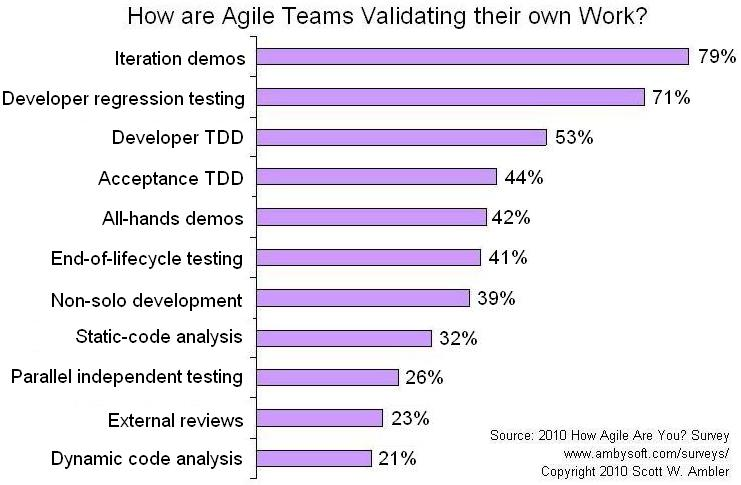
\includegraphics[scale=.4]{agileCriteria2010Validating}
    \caption{Como times ágeis validam seu próprio trabalho?}
    \label{fig:wambler-agile-2010}
  \end{minipage}
  \hspace{0.5cm}
  \begin{minipage}[b]{0.45\linewidth}
    \centering
    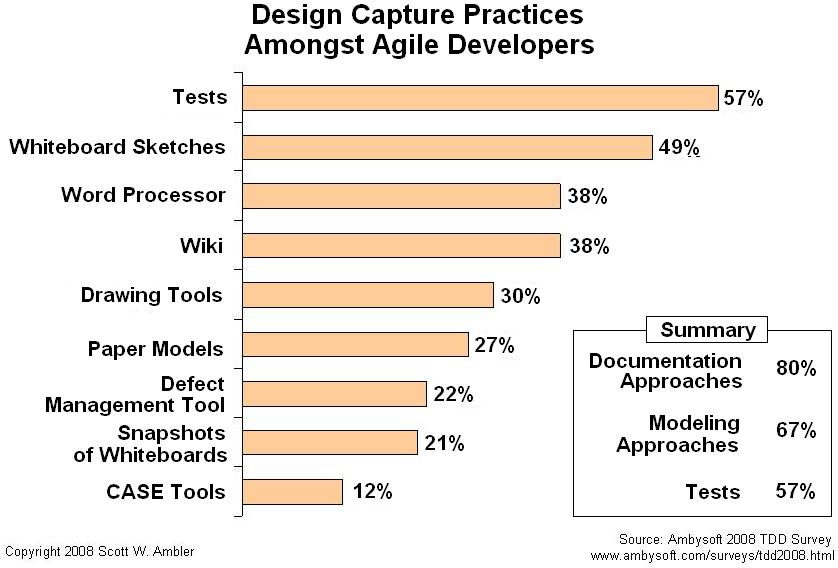
\includegraphics[scale=.35]{tddDesignPractices}
    \caption{Práticas que desenvolvedores ágeis usam para auxiliar no design}  
    \label{fig:wambler-tdd-2008}
  \end{minipage}
\end{figure}			

%% ------------------------------------------------------------------------- %%
\section{Motivação}

A motivação desta pesquisa é a crescente popularidade de TDD, tanto na
academia quanto na indústria, e a pouca quantidade de trabalhos
voltados a entender como a prática influencia as decisões de 
design no dia a dia do desenvolvedor.

Para o desenvolvedor, Ao entender melhor essas influências de design, 
ele pode melhorar, maximizar o retorno ou até mesmo adaptar a prática.

Para a indústria, é importante conhecer os reais efeitos de TDD no design,
e esse trabalho pode servir de apoio à decisão da adoção da prática
de TDD nos times de desenvolvimento.

%% ------------------------------------------------------------------------- %%
\section{Contribuições}

Este trabalho
visa compreender a real influencia de TDD no design de classes.
Mais profundamente, este trabalho avalia a relação entre a prática de 
TDD
e as decisões de design tomadas pelos desenvolvedores no processo de 
criação de classes.

A análise será feita por meio de dados que serão
capturados baseados na percepção de programadores atuantes na indústria, após
a implementação de alguns pequenos problemas especialmente criados para
esta pesquisa.

Os objetivo principal deste estudo é \textbf{entender a relação da prática de TDD 
e as decisões de design tomadas pelo programador durante o processo de 
design de sistemas orientados a objetos}.
Para compreendê-la, tenta-se responder às questões listadas
abaixo:

\begin{enumerate}

	\item Qual a influência de TDD no design de classes?

	\item Qual a relação entre TDD e as tomadas de decisões de design
	feitas por um desenvolvedor?

	\item Como a prática de TDD influencia o programador no processo de  
	design de classes, do ponto de vista do acoplamento, coesão e simplicidade?

\end{enumerate}

%% ------------------------------------------------------------------------- %%
\section{Organização do trabalho}

Este trabalho está dividido da seguinte maneira: 

\begin{itemize}
	\item O Capítulo \ref{cap:tdd} discute sobre a prática de TDD, com ênfase no
	ponto de vista do design;
  
	\item O Capítulo \ref{cap:trabalhos-relacionados} mostra trabalhos já
	realizados pela academia sobre os efeitos de TDD;

 	\item O Capítulo \ref{cap:qualitativo} discute métodos qualitativos de
 	pesquisa e suas características;

	\item O Capítulo \ref{cap:planejamento} discute o planejamento do experimento,
	bem como o processo de captura de dados e análise;

	\item O Capítulo \ref{cap:discussao} apresenta os resultados encontrados e
	os discute;
	
	\item O Capítulo \ref{cap:ameacas} discute as possíveis ameaças aos resultados
	encontrados na pesquisa;
	
	\item O Capítulo \ref{cap:conclusoes} resume o trabalho realizado e apresenta
	possibilidades de trabalhos futuros.
\end{itemize}

